\documentclass[12pt,a4paper]{article}

\usepackage{geometry}
\geometry{
  a4paper,
  total={170mm,257mm},
  left=20mm,
  right=20mm,
  top=20mm
}

\usepackage[utf8]{inputenc}
\usepackage[english, greek]{babel}
\usepackage[LGR, T1]{fontenc}

\usepackage{amsmath}
\usepackage{amsfonts}

\usepackage{tikz}
\usetikzlibrary{arrows.meta,automata,positioning}

\usepackage{titlesec}
\titleformat{\section}{\large}{}{0em}{\textsc}[\titlerule]
\titleformat{\subsection}{\large}{}{0em}{\textbf}[]
\titleformat{\subsubsection}{}{}{0em}{\textit}[]

\title{Αλγόριθμοι και Πολυπλοκότητα}
\author{Γαβαλάς Νίκος, AM 03113121}
\date{Δεκέμβριος 2018}

\begin{document}

  \maketitle

  \begin{center}
    \Large{3η Γραπτή Σειρά Ασκήσεων}
  \end{center}

  \section{Άσκηση 1}

  \section{Άσκηση 2}

  Έχουμε γράφο \( G(V, E) \) με \( p(u) \in \mathbb{N}, u \in V \) και ζητάμε 
  την τιμή  \( c(u), \forall u \in V \), όπου \( c(u) \) είναι η τιμή της 
  φθηνότερης κορυφής που είναι προσπελάσιμη από τη \( u \), μαζί με τη \( u \).

  \subsection{α}

  Aν ο γράφος \( G \) είναι {\latintext DAG}, γνωρίζουμε πως τότε ορίζεται
  τοπολογική διάταξη μεταξύ των κορυφών του, η οποία σχηματίζεται σε χρόνο
  \( Ο(|V| + |E|) \) (γραμμικό).
  \\
  \\
  Διατάσσουμε λοιπόν τις κορυφές και ύστερα,
  προσπελαύνοντας τες αντίστροφα, κρατάμε για κάθε μία τη μικρότερη τιμή
  \( c(u) \) βάσει της σχέσης \( c(u) = \min\{ p(u), \min_{ v : (u, v) \in E}
  \{c(v)\}\} \).
  \\
  \\
  Το δεύτερο βήμα απαιτεί επίσης γραμμικό χρόνο, επομένως ο αλγόριθμος είναι
  γραμμικού χρόνου.

  \subsection{β}

  Γνωρίζουμε ότι κάθε γράφος μπορεί να παρασταθεί ως {\latintext DAG} των 
  {\latintext SCC} του, σε γραμμικό χρόνο.
  \\
  \\
  Κάθε κορυφή \( u \in W \), \( W \) {\latintext SCC} του \( G \),
  θα έχει την ίδια τιμή \( c(u) \) με τις υπόλοιπες κορυφές που
  ανήκουν στην ίδια {\latintext SCC}, αφού ακριβώς επειδή είναι ισχυρά συνεκτική
  συνιστώσα και άρα υπάρχει διαδρομή από και προς οποιοδήποτε
  \( u, v \in W \), αρκεί να
  βρούμε την ελάχιστη \( p(u) \) μεταξύ όλων αυτών και ύστερα σε όλες θα θέσουμε
  \( c(u) \) ίση με αυτήν.
  \\
  \\
  Αρχικά, βρίκουμε λοιπόν τις {\latintext SCC}, και για κάθε μία \( W \) από
  αυτές υπολογίζουμε την ελάχιστη τιμή μεταξύ όλων των κορυφών \( u \in W \),
  δηλαδή το \( P(W) = \min_{u \in W}\{ p(u) \}\).
  \\
  \\
  Στη συνέχεια, σχηματίζουμε τον μεταγράφο που αποτελεί το {\latintext DAG} των 
  {\latintext SCC \( W \)} του \( G \), και τρέχουμε τον αλγόριθμο του
  ερωτήματος (α) υπολογίζοντας τις τιμές \( C(W) \) με βάση τα \( P(W) \).
  \\
  \\
  Tέλος, για κάθε {\latintext SCC \(W\)}, για κάθε κορυφή \(u \in W \), θέτουμε
  \( c(u) = C(W) \).
  \\
  \\
  Η χρονική πολυπλοκότητα του αλγορίθμου είναι γραμμική, αφού κάθε βήμα απαιτεί
  χρόνο \( Ο(|V| + |E|) \).

  \section{Άσκηση 3}
  
  \section{Άσκηση 4}

  Έστω συνεκτικός, μη κατευθυνόμενος γράφος \( G(V, E) \) με \( |V| = n,
  |E| = m \).

  \subsection{α}

  Έστω \(T_1, T_2\) συνεκτικά δέντρα και ακμή \(e' \in T_2 \backslash T_1\).
  To \(T_1 \cup \{e'\}\) θα περιέχει κύκλο \(C\). Σε αυτόν τον κύκλο, \(\exists
  e \in C: e \notin T_2\), αφού διαφορετικά το \(Τ_2\) θα περιείχε τον \(C\)
  και δεν θα ήταν συνδετικό δέντρο. Το \((T_1 \backslash \{e\}) \cup \{e'\} \)
  είναι άκυκλος γράφος με \(|E| = |V| - 1\), άρα είναι συνδετικό δέντρο.
  Επομένως, \(\forall e \in T_1 \backslash T_2, \exists e' \in T_2 \backslash
  T_1: (T_1 \backslash \{e\}) \cup \{e'\}\) είναι συνδ. δέντρο.
  \\
  \\
  Μια τέτοια ακμή μπορεί να βρεθεί σε γραμμικό χρόνο ως εξής: για \(e = (u, v)
  \in T_1 \backslash T_2 \), πραγματοποιούμε στο \(T_2 \) μια {\latintext DFS}
  αναζήτηση από το \(u \rightarrow v\) και για κάθε ακμή \(e'\) που ανήκει στο
  προκύπτον μονοπάτι εξετάζουμε αν \(\in Τ_1\) σε \((O(1))\) και επιστρέφουμε 
  την πρώτη που \(\notin T_1\). Η πολυπλοκότητα είναι αυτή του {\latintext DFS},
  \(O(|V|)\).
  
  \subsection{β}

  \subsection{γ}

  \section{Άσκηση 5}

  Έστω \(G(V, E, w)\) συνεκτικός και μη κατευθυνόμενος γράφος.

  \subsection{α}

  \begin{center}
    \begin{tabular}{c c}
      \underline{Γράφος} & {\latintext \underline{MST}} \\
      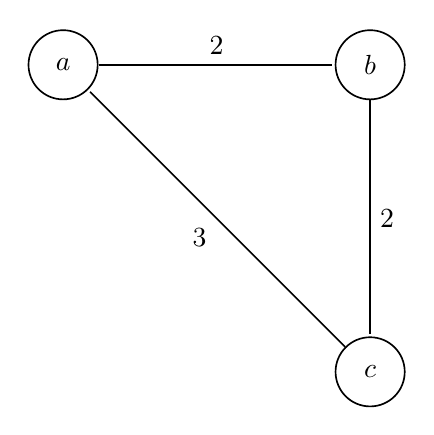
\begin{tikzpicture}[
        > = stealth, % arrow head style
        shorten > = 1pt, % don't touch arrow head to node
        auto,
        node distance = 3cm, % distance between nodes
        semithick % line style
        ]
    
        \tikzset{every state}=[
        draw = black,
        thick,
        fill = white,
        minimum size = 1mm
        ]
    
        \node[state] (a) {\(a\)};
        \node[state] (b) [right=of a] {\(b\)};
        \node[state] (c) [below=of b] {\(c\)};
    
        \path[] (a) edge  node[] {2} (b);
        \path[] (b) edge  node[] {2} (c);
        \path[] (c) edge  node[] {3} (a);
    
      \end{tikzpicture} &
      \begin{tikzpicture}[
          > = stealth, % arrow head style
          shorten > = 1pt, % don't touch arrow head to node
          auto,
          node distance = 3cm, % distance between nodes
          semithick % line style
          ]
      
          \tikzset{every state}=[
          draw = black,
          thick,
          fill = white,
          minimum size = 1mm
          ]
      
          \node[state] (a) {\(a\)};
          \node[state] (b) [right=of a] {\(b\)};
          \node[state] (c) [below=of b] {\(c\)};
      
          \path[] (a) edge  node[] {2} (b);
          \path[] (b) edge  node[] {2} (c);
      
        \end{tikzpicture}
    \end{tabular}
  \end{center}

  \subsection{β}

  Αφού για κάθε τομή, η ακμή ελάχιστου βάρους που διασχίζει την τομή είναι
  μοναδική, τότε όλες οι ακμές θα έχουν διαφορετικά βάρη, γιατί αν υπήρχαν
  τουλάχιστον δύο ακμές με το ίδιο βάρος θα υπήρχε τομή για την οποία από
  τις διασχίζουσες ακμές είτε θα υπήρχε μικρότερη (οπότε δεν μας νοιάζει), ή
  θα ήταν και οι δύο οι μικρότερες (εφόσον είναι ίσες) και άρα δεν θα υπήρχε
  μοναδική ακμή ελάχιστου βάρους. Συνεπώς, γνωρίζοντας πως όταν σε συνδετικό μη
  κατευθυνόμενο γράφο όλες οι ακμές έχουν διαφορετικά βάρη, τότε το
  {\latintext MST} του γράφου είναι μοναδικό, προκύπτει το ζητούμενο.
  \\
  \\
  Αντιπαράδειγμα:
  \\
  \begin{center}
    \begin{tikzpicture}[
      > = stealth, % arrow head style
      shorten > = 1pt, % don't touch arrow head to node
      auto,
      node distance = 3cm, % distance between nodes
      semithick % line style
      ]
  
      \tikzset{every state}=[
      draw = black,
      thick,
      fill = white,
      minimum size = 1mm
      ]

      \node[state] (a) {\(a\)};
      \node[state] (b) [right=of a] {\(b\)};
      \node[state] (c) [below=of b] {\(c\)};

      \draw[red,thick,dashed] (3,1) .. controls (2.5,-1.5) .. (6,-1);
  
      \path[] (a) edge  node[] {2} (b);
      \path[] (b) edge  node[] {2} (c);
      \path[] (c) edge  node[] {3} (a);
  
    \end{tikzpicture}
    
  \end{center}
  \subsection{γ}

  \subsection{δ}

\end{document}
